With our background in both medical procedures and machine learning, we can now look at how we want to solve the problems associated with setting up a system for medical diagnosis.  
We will first get a birds-eye view of the objective of this thesis, looking at the hypothesises presented in the introduction, and take a look into how we can test their validity. We look at the proposed program set up to test the hypothesises both for classification and generation.
Then we look at the language and packages suitable for this project. We go in-depth into the reasoning behind why we chose the tools and packages that became the foundation of the programs. We end the chapter by presenting the program designed to test our problem statements.


\section{Bird's Eye View}
\label{cha:BEW}
In the summary of the background chapter, we looked at two articles published by Pogorelov et al. and Hicks et al. where they discussed the effect of overfitting and the consequences of dataset-specific artefacts.
To help solve these predicaments look back at the two hypothesises presented in section~\ref{cha:problemstatement}:

\vspace{2px}
Hypothesis~\ref{hyp:a} stated that sparse information in the images made it harder to classify the images correctly. Figure \ref{fig:Saliencymasks} from Hicks's paper shows the case where the black areas with sparse information activates the classification map. As we can see, the black areas trigger as a ``positive'' in some om the saliency maps. We can interpret this as the network learning features not useful for the classification. 
Our quest is to check the validity of hypothesis \ref{hyp:a}. We propose to test the classification of images with and without areas with sparse information by inpainting the images.


\vspace{5px}
Hypothesis~\ref{hyp:b} stated that dataset specific artefacts create false positives and negatives. This error is clearly shown in \ref{fig:sal2}, where the classification is affected by the green square in the image. 
As long as the classification is affected by dataset specific artefacts, the ability to adapt the dataset to new use cases might suffer.  


\begin{figure}[t]
     \centering
     \begin{subfigure}[t]{0.3\textwidth}
         \centering
         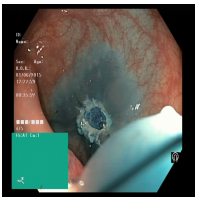
\includegraphics[width=\textwidth]{methodology/figures/sal1.png}
         \caption{Original image}
         \label{fig:sal1}
     \end{subfigure}
     \hfill
     \begin{subfigure}[t]{0.3\textwidth}
         \centering
         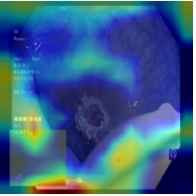
\includegraphics[width=\textwidth]{methodology/figures/sal2.png}
         \caption{Heatmap}
         \label{fig:sal2}
     \end{subfigure}     
     \hfill
     \begin{subfigure}[t]{0.3\textwidth}
         \centering
         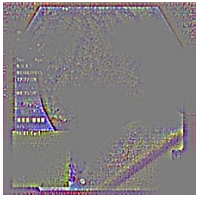
\includegraphics[width=\textwidth]{methodology/figures/sal3.png}
         \caption{Saliency map}
         \label{fig:sal3}
     \end{subfigure}
     \caption{Heat and Saliency maps of an unaugmented dataset where the images are generated by Mirmir}
     \label{fig:Saliencymasks}
\end{figure}

\begin{figure}[t]
     \centering
     \begin{subfigure}[t]{0.3\textwidth}
         \centering
         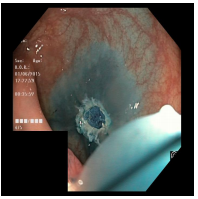
\includegraphics[width=\textwidth]{methodology/figures/sal4.png}
         \caption{Augmented image}
         \label{fig:sal4}
     \end{subfigure}
     \hfill
     \begin{subfigure}[t]{0.3\textwidth}
         \centering
         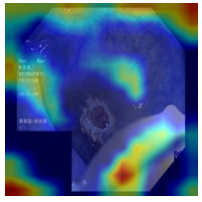
\includegraphics[width=\textwidth]{methodology/figures/sal5.png}
         \caption{Heatmap}
         \label{fig:sal5}
     \end{subfigure}     
     \hfill
     \begin{subfigure}[t]{0.3\textwidth}
         \centering
         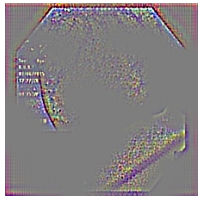
\includegraphics[width=\textwidth]{methodology/figures/sal7.png}
         \caption{Saliency map}
         \label{fig:sal7}
     \end{subfigure}
     \caption{Heat and Saliency maps of an augmented dataset where the green corner is removed. The images are generated by Mirmir}
     \label{fig:Saliencymasks2}
\end{figure}



We note that \ref{hyp:a} concerns both training and testing on the same dataset, while \ref{hyp:b} is more concerned about the generalisability of the model, and hence the goal is to use different datasets for training and testing, as well as testing on the training set. 


To test the two hypotheses, we first need new datasets to compare against a base case. In addition to the dataset with sparse information and dataset-specific artefacts, we need similar looking datasets without these unwanted features. In an ideal scenario, we would have the same dataset without the features added post-capture. 

In the real world, gathering labelled data is often both a challenging and expensive task. In this thesis, we have decided to focus our attention at modifying existing data instead of finding new data. 
We propose to use unsupervised machine learning to inpaint the areas with dataset specific artefacts as well as sparse areas. We then propose a transfer learning network to classify the newly created images. 


\section{Design of the Inpainting Algorithms}

We first want to set up a platform where every dataset is made with the same parameters, except for the dataset-specific parameters that define the dataset. 
When generating the datasets, we use the Kvasir dataset~\cite{Pogorelov:2017:KMI:3083187.3083212} as the training set, as Hicks et al. did in their paper on removing dataset specific artefacts~\cite{25956}. In addition, we use datasets without the artefacts for testing.
This selection of image sources was made intentionally to have a fundamentally different test and training set, and the more differences between testing and training set the more of an indication of generalisation. 

Figure \ref{fig:KvasirAnomaliesFIX} shows two different image types from the Kvasir dataset. 
Figure \ref{fig:LargeLeftBlack} shows an image of esophagitis. This image shows one of the main problems with the Kvasir dataset when it comes to artefacts. In addition to the cut corners, we have an extra wide area to the left of the image containing non-relevant information like name, sex, and other comments. This area gives us ample opportunity to test hypothesis \ref{hyp:a}, given that the image contains a large amount of sparse information that we want to remove to see the effect on classification. 
We believe that if we can change images like the one in Figure \ref{fig:LargeLeftBlack} into images like the one in Figure \ref{fig:LargeLeftBlackFIX}, we will see an improvement in classification when testing and training on the same dataset.

Figure \ref{fig:GreenSquareOccluding} shows another problem with datasets like Kvasir.  Here we have a green square in the bottom left corner that occludes parts of the image and the same type of text displaying name age and other non-relevant information. We recall from section \ref{cha:BEW} that information like this can give the classifier false positives, and subsequently provide us with a lower classification score. 
We believe that if we can change images like the one in Figure \ref{fig:GreenSquareOccluding} into images like the one in Figure \ref{fig:GreenSquareOccludingFIX} we will see an improvement in classification when testing and training on different datasets.


\begin{figure}
     \centering
     \begin{subfigure}[t]{0.4\textwidth}
         \centering
         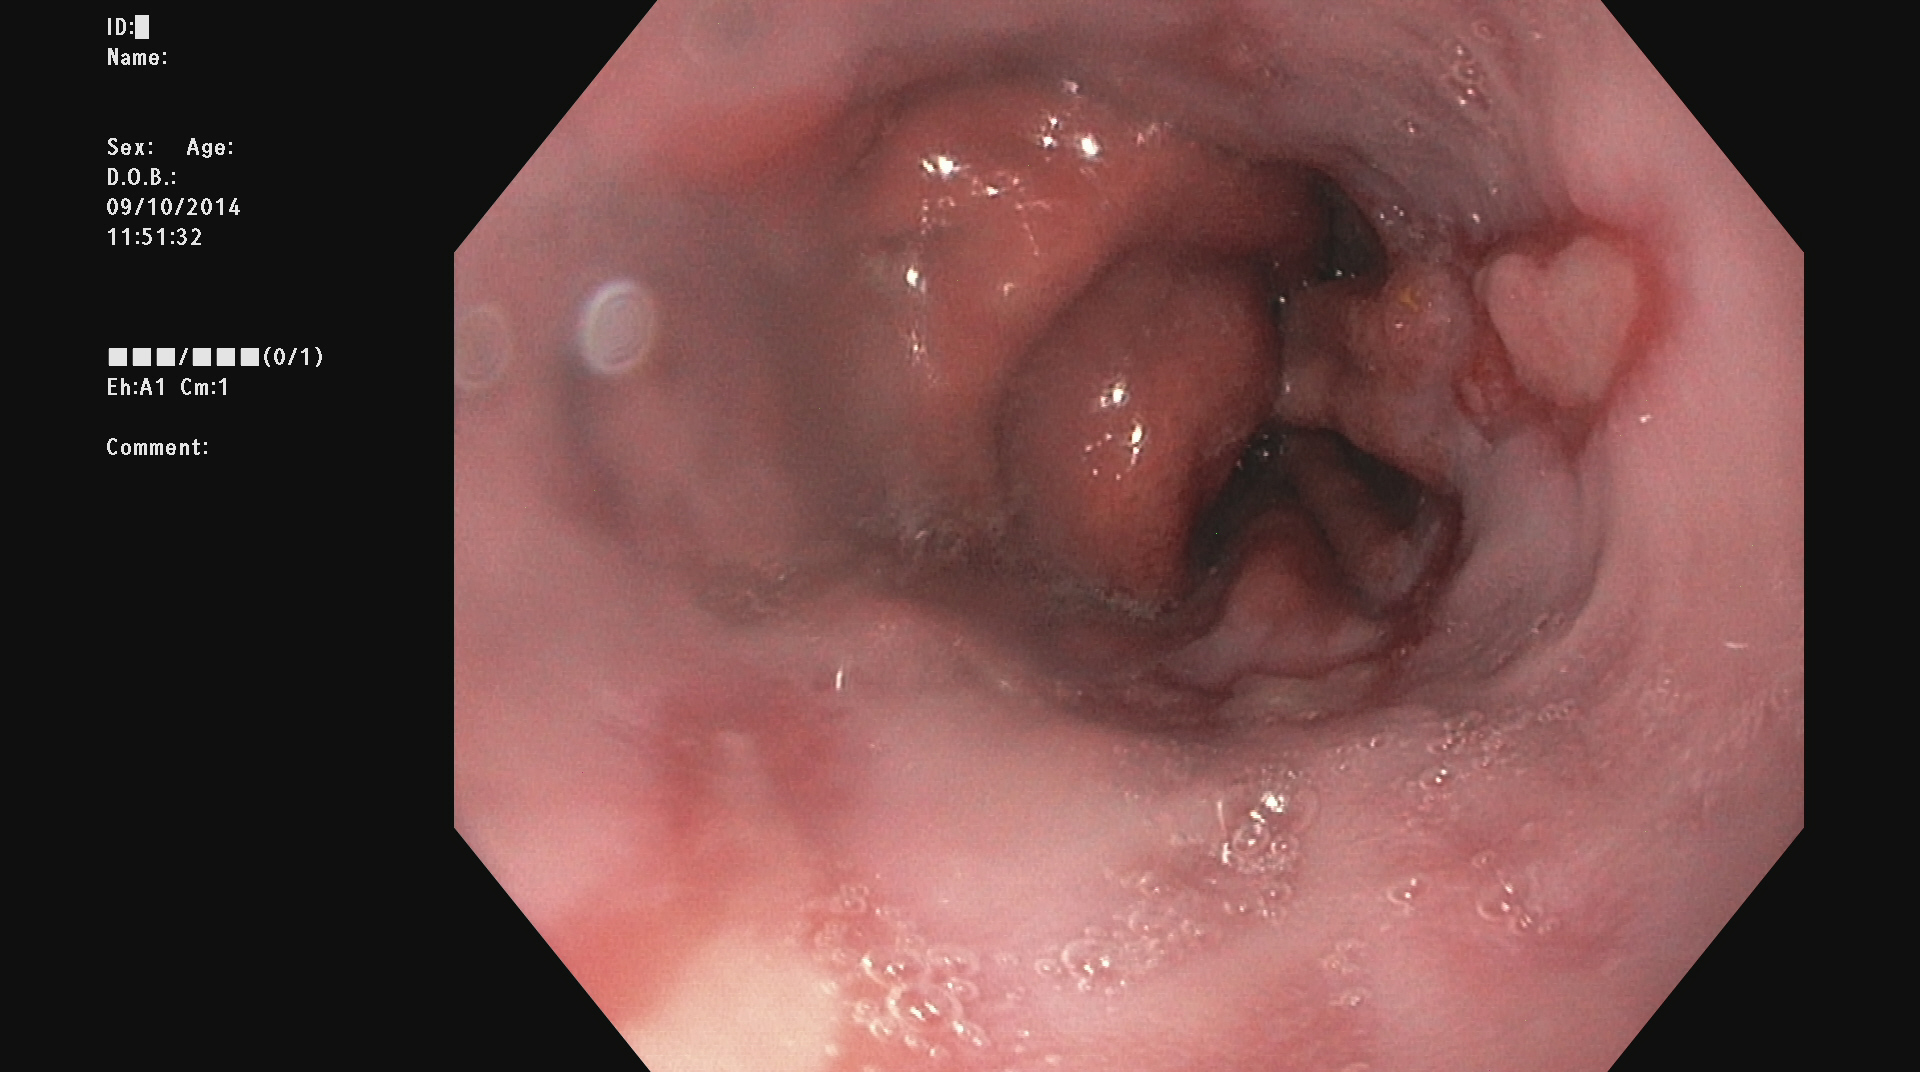
\includegraphics[height=\textwidth, width=\textwidth]{experiments/figures/leftframe.jpg}
         \caption{Example of an image with a large area without relevant medical information}
         \label{fig:LargeLeftBlack}
     \end{subfigure}
     \hfill
     \begin{subfigure}[t]{0.4\textwidth}
         \centering
         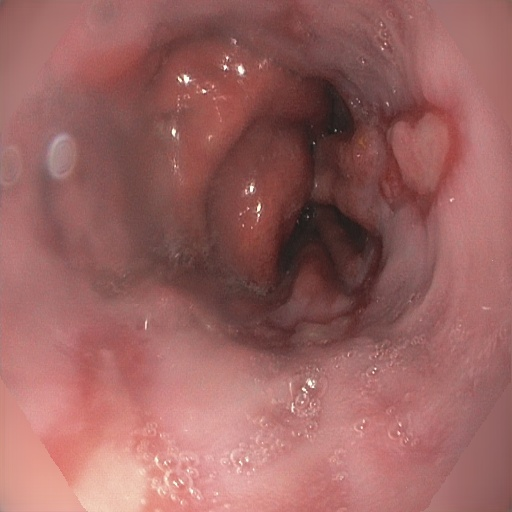
\includegraphics[height=\textwidth, width=\textwidth]{experiments/figures/noleftframe.jpg}
         \caption{The same image as in Figure \ref{fig:LargeLeftBlack} with the non-relevant information removed}
         \label{fig:LargeLeftBlackFIX}
     \end{subfigure}
     \hfill
     \begin{subfigure}[t]{0.4\textwidth}
         \centering
         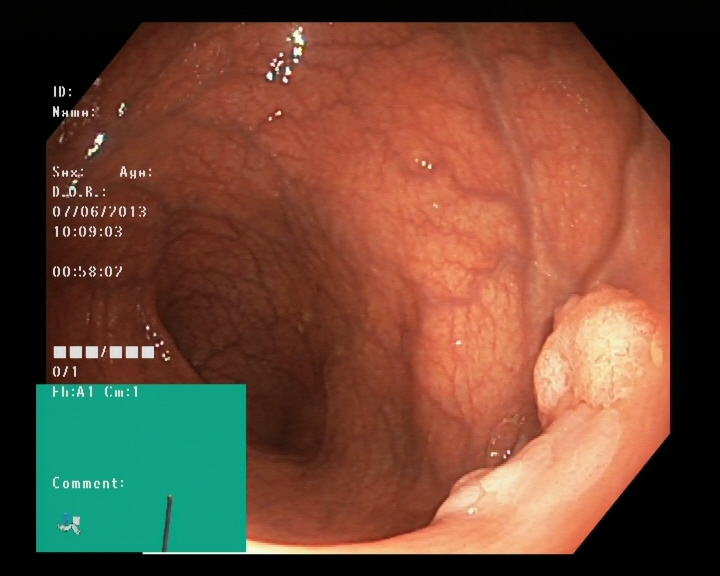
\includegraphics[height=\textwidth, width=\textwidth]{experiments/figures/greenframe.jpg}
         \caption{Example of an image with green square occluding the parts of the GI tract}
         \label{fig:GreenSquareOccluding}
     \end{subfigure}     
     \hfill
     \begin{subfigure}[t]{0.4\textwidth}
         \centering
         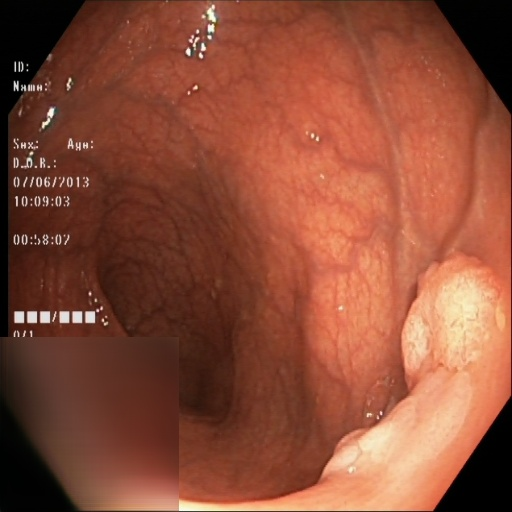
\includegraphics[height=\textwidth, width=\textwidth]{experiments/figures/nogreenframe.jpg}
         \caption{The same image as in Figure \ref{fig:GreenSquareOccluding} with the green square inpainted}
         \label{fig:GreenSquareOccludingFIX}
     \end{subfigure}
        \caption{Images where the troubling areas are removed before training}
        \label{fig:KvasirAnomaliesFIX}
\end{figure}


We propose three different types of inpainting to prove or disprove our two hypothesises.
\FloatBarrier
\subsection{Removing black corners}
The most straightforward experiment to conduct is to test how the removal of the black corners will affect the result.
As we propose in hypothesis \ref{hyp:a}, we believe that this masking can help giving the classifier fewer areas with non-relevant information.
Figure \ref{fig:CornerMask} shows the mask used to inpaint the corners.

As we recall from section \ref{cha:endocolo}, the black edges around the images in our datasets is also, in general, present in medical colonoscopy images. By removing the black corners around the image, we do not change \textit{Kvasir specific} artefacts, but according to our first hypothesis, we believe we will get a higher classification accuracy since this removes areas with sparse information.

When classifying images during the testing stage, we need to take inpainting during training into account. 
\begin{enumerate}
\item We can do the same masking and inpainting on the test set. 
\item We can crop the image in a way that removes the black corners without inpainting.
\item We can forgo modifying the test data and just run the test set as is. 
\end{enumerate}


\paragraph{Method 1}
We tested method 1) in our paper ``Using preprocessing as a tool in medical image detection''~\cite{26254}.
The goal of this paper was related to hypothesis \ref{hyp:a} with the fact that we wanted to see how removing areas with sparse information affected the result of classification when training and testing on similar datasets. 
In the experiments run within this paper, both the training set and test set were inpainted. 
Since the focus of this task was to classify a test set we had from beforehand correctly, we had the option to preprocess the test set in addition to the training set without any penalties based on time restrictions. 
Our paper inpainted the test set as proposed in method 1) and from the results, it showed minimal improvement. The lack of improvement is mainly not connected to the fact that we inpainted the test set, but the fact that the test set came from the same distribution as the training set, and subsequently ended up with a model that overfitted to the data.
Given that we, in the end, want to classify images from a live colonoscopy, we have decided to forgo the inpainting of the test set using method 1).
By not augmenting the test set the experiments are also suited to reflect a larger research area of machine learning.



\paragraph{Method 2}
Method number 2) was the proposal of cropping the images during evaluation.  Thambawita et al. did similar methods in the Mediaeval 2018 conference but also had the same cropping during training. In the paper ``The Medico-Task 2018: Disease Detection in the Gastrointestinal Tract using Global Features and Deep Learning''~\cite{26205} we can see that this method worked with great success. 
The operation of just cropping images is also multiple times as fast as inpainting images, so it is feasible for a live recording. 

One of our four test cases in our first publication looked into cropping the images to the extent that we removed the black corners completely~\cite{26254}. The result from our tests showed the lowest classification score, far below the baseline of comparison, giving us the impression that our extensive cropping removed essential parts of the image. 
The downside of cropping the images from the test set is the fact that we do not have control over what we remove from the data. Given that the test set might come from a completely different distribution, we might unwillingly remove information we desire to keep. We do also run into the problem that cropping the images are not feasible when the sparse areas are within the image, and not at the outer edges.

\paragraph{Method 3}
The last proposed method is not to augment the images during testing. This method, since we are not preprocessing the test data at all, is the fastest when it comes to live classification. Without the augmentation, we risk getting a lower classification score, but we do not remove any data. Also, we make our results better reflect on how it will work on non-medical datasets.\\

\noindent
In this thesis we will use method number 3. 

We base this decision on that we want the final product to have the option to be used live and be easily adaptable to other datasets. 
Method number 3) also coincides with the method used in our second paper, \textit{``Unsupervised preprocessing to improve generalisation for medical image classification''}~\cite{Mathias2019IEEpaper}. By using the same inpainting methods for the test set as in our published paper, we can reasonably draw direct comparisons.
An important note here is that the datasets in the thesis and the published paper are the same, though the method for achieving the results differ.


%w
\subsection{Removing the Green Square}
The next major area in question is the removal of the green squares located in the bottom left area of some of the medical images.  This area is a Kvasir specific artefact and is found in 38\% of the images spanning five out of eight classes. 
By inpainting the lower left area we can see if our hypothesis \ref{hyp:b} is correct since here we are removing a dataset-specific feature that the network can use to determine classes. 
We have also chosen to inpaint every image, regardless of the green square is there or not. We do this so that the network can not ``learn'' that the pattern from the inpainted area correlates with the five classes with the green square, and hence defeating the purpose of the inpainting. Figure \ref{fig:GreenMask} shows the mask used to inpaint the lower left corner.

When classifying images during the testing stage, we have the same decision to take when it comes to inpainting of the test set.
\begin{enumerate}
\item We can either do the same masking and inpainting on the test set. 
\item We can crop the image in a way that removes the dataset-specific artefacts.
\item We can forgo modifying the test data and just run the test set as is. 
\end{enumerate}

To keep the consistency between the two different inpainting methods, we use method 3) for the test set.
As with the black corners to be inpainted, we choose not to preprocess the test data, as this takes time, and should in theory not be necessary to get the right classification.
 

\subsection{Removing Both Corners and the Green Square}
The last set we want to test is the combination of both inpainting the green square and the black corner as shown with the mask in Figure \ref{fig:BothMask}. 
Here we hope that a combination of hypothesis \ref{hyp:a} and \ref{hyp:b} will give the strength of both methods without any harmful interference. 

\subsection{Removal of Over-saturated Areas and Text}
To thoroughly test the hypothesis \ref{hyp:b} we should also remove areas that are not always found in the same area each time. Text and over-saturated pixels can, in the Kvasir dataset, be at any region, making the inpainting task less trivial. 

To remove those kinds of artefacts, other methods to locate the areas are also needed. We conducted experiments using Google's Tesseract OCR~\cite{smith2007overview} to locate text, though, the time it took to find the areas made it not feasible for training. 
In the finished product, we do not remove that kind of artefacts, given the complexity of the problem coupled with the relatively small size of the artefacts in question.

\subsection{The Generative Modelling Algorithms}
With the three masks discussed, we now want to present the generative modelling algorithms. As addressed in section \ref{cha:BEW} our goal is to make new datasets without the unwanted artefacts based on the original dataset. 
We have chosen to use the two generative models presented in section \ref{cha:Explaining_autoencoders} and in section \ref{cha:Explaining_GANS}, namely Autoencoders and GANs.


As we recall from section \ref{cha:Explaining_autoencoders} the autoencoder and GAN\footnote{It is necessary to mention that regular GANs does not use a ground truth when training, though our modified GAN do.} networks both use a ground truth when training.
When training we need images that are already inpainted as a reference point. We solve this by zooming in the images to the limit that the edges are gone, as shown in figure \ref{fig:CornerMask}. When removing the dataset-specific features, we have the luxury that not all images contain the green square, giving us ample data for training after the images are sorted.
By removing the corners by zooming and by using images without artefacts during training, we have images where we know the whole ground truth, giving us the option to use MSE for backpropagation.


When training the GAN, we often do not need a ground truth behind the mask, as the network only tries to discern if the image is real or fake. This gives us in practice the same restrictions as with backpropagating with MSE.

\subsection{Summary}
We have now talked about the three main masks we use, combined with the two generative models that make the datasets.
In total, we end up with six generated datasets, two for each mask type, and one unaugmented base case.
The seven datasets will be the basis for our test of the problem statements. 



\begin{figure}[h]
     \centering
     \begin{subfigure}[t]{0.37\textwidth}
         \centering
         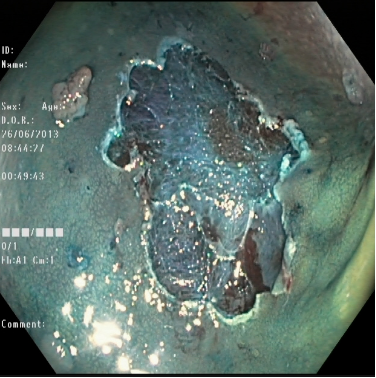
\includegraphics[width=\textwidth]{methodology/figures/nomask.png}
         \caption{Image from the original non-augmented dataset}
         \label{fig:CornerMask}
     \end{subfigure}
     %\hfill
     \hspace*{2cm}
     \begin{subfigure}[t]{0.37\textwidth}
         \centering
         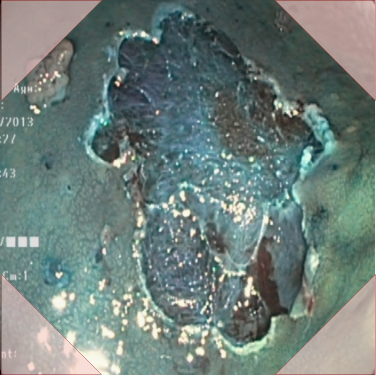
\includegraphics[width=\textwidth]{methodology/figures/cornermask.png}
         \caption{Red area shows the area masked in the first of the generated datasets}
         \label{fig:CornerMask}
     \end{subfigure}
     %\hfill
     \begin{subfigure}[t]{0.37\textwidth}
         \centering
         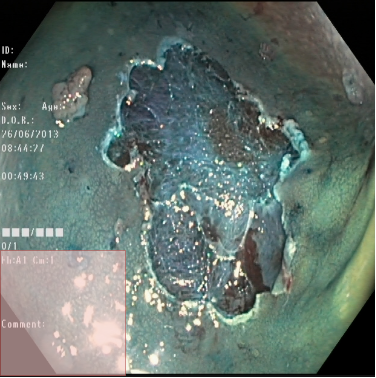
\includegraphics[width=\textwidth]{methodology/figures/greenmask.png}
         \caption{Red area shows the area masked by the second of the datasets}
         \label{fig:GreenMask}
     \end{subfigure}     
     %\hfill
     \hspace*{2cm}
     \begin{subfigure}[t]{0.37\textwidth}
         \centering
         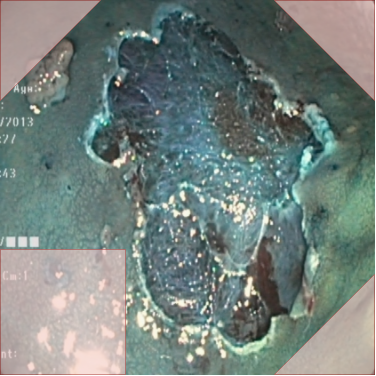
\includegraphics[width=\textwidth]{methodology/figures/bothmask.png}
         \caption{Red area shows the area masked by the third of the datasets}
         \label{fig:BothMask}
     \end{subfigure}
     \caption{All three mask types used in this thesis, and associated images used during training. The different masks require different levels of cropping, as shown in the subfigures.}
     \label{fig:masks}
\end{figure}


\FloatBarrier
\section{Design of the Transfer Learning Experiments}
\label{cha:classifier}
To test the hypothesises we need a system in place to compare the datasets we generate with inpainting. As we recall, we base both our hypothesis on an improvement compared to the original dataset we provide. 
To see if we have any improvement we propose to use a classifier based on transfer learning to see how the newly generated datasets give a better classification score compared to the base dataset without augmentations.

We want to test our system with a range of different models and classifiers to test the validity of the system and to make sure that our results are not just good outliers.

Figure \ref{fig:KTLmodel} shows the general structure of the transfer learning model we use in this thesis. 

Hyperparameter optimisation of the models is a challenging task~\cite{runeMedico2018}. In this thesis, we have chosen to use automatic hyperparameter optimisation provided by the hyperparameter optimiser made by Borgli et al. in the MediaEval workshop 2019~\cite{runeMedico2018}, to give us the optimal model for training. Based on our dataset, the optimal network, DenseNet121~\cite{DBLP:journals/corr/HuangLW16a}, was chosen as our primary model for evaluation. 
In addition to an optimal model, we have chosen to use InceptionResNetV2~\cite{DBLP:journals/corr/SzegedyIV16} as a more general model. InceptionResNetV2 showed the highest top 1 and top 5 accuracies on imagenet when we designed the transfer learning program based on the Keras website in August 2018. We find a more recent table with more pretrained models in Figure \ref{tab:Kaeras_app}.


\begin{figure}[t]
        \centering
        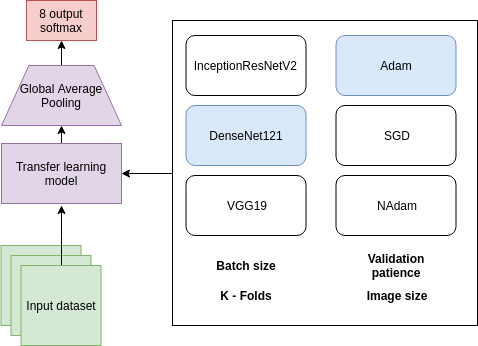
\includegraphics[scale=0.47]{methodology/figures/model.png}
        \caption{ The model we use for classifying with the most important options for the learning process. }
    \label{fig:KTLmodel}
\end{figure}



\subsection{Models}
The models used in the evaluation of our results are fundamentally different from one another, and to better understand the results we give a short introduction of both pretrained networks. 

\paragraph{Inception Residual Network architecture }
We can often see performance gains in our network architectures when we increase the size of the network. To increase the size, we can either increase the depth of the network, i.e. the number of layers, or we can increase the width of the network, i.e. increase the number of units per layer. Both methods are often easy to implement, but it often comes with the drawback of either increasing the number of parameters to train, which can result in overfitting, or it can result in the computation time of the network to increase to an undesirable length.
To find a balance between accuracy and memory is often a hard task when it comes to not only medical images but images in general.

Szegedy et al. presented an architecture for the imagenet challenge with the intention of reducing the computational cost of training large neural networks by decreasing the number of parameters~\cite{DBLP:journals/corr/SzegedyLJSRAEVR14}. 
The network presented, GoogLeNet, used inception modules to reduce the computational cost.  Inception modules (networks within networks) tries to answer the question of witch convolution is the correct for each layer. Often it is up to the network architect to decide this, but with inception modules, the network chooses for itself. 
In the GoogLeNet paper, the inception modules are the same as in Figure \ref{fig:Inception}, showing the option between $1 \times 1$, $3 \times 3$, $5 \times 5$ convolutions, and $3 \times 3$ max pooling, followed by a concatenation of the four options. In addition to the convolution in parallel, the original authors added $1 \times 1$ convolution before the larger filters. This layer uses 128 filters that are designed to reduce the dimensionality if the network, and subsequently, reduce the number of parameters in the network.


Microsoft proposed another solution to training very deep neural networks in the form of residual modules~\cite{DBLP:journals/corr/HeZRS15} as shown in Figure \ref{fig:Residual}.
When using sufficiently large enough networks the backpropagation often encounter the problem with vanishing gradients. By adding a direct link between the layers, we counteract the vanishing gradient problem. A consequence we encounter when using residual modules is that instead of recreating the input for each layer, each layer learns only to modify the input value instead of completely recreating it.

\begin{figure}
     \centering
     \begin{subfigure}[t]{0.4\textwidth}
         \centering
         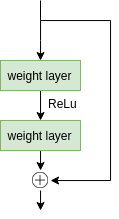
\includegraphics[width=0.5\textwidth]{methodology/figures/residual.png}
         \caption{Residual module concept as proposed in~\cite{DBLP:journals/corr/HeZRS15}}
         \label{fig:Residual}
     \end{subfigure}
     \hfill
     \begin{subfigure}[t]{0.55\textwidth}
         \centering
         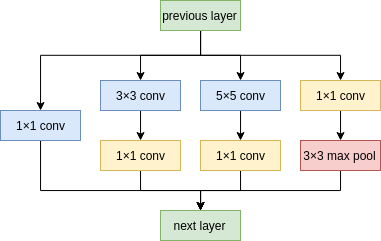
\includegraphics[width=\textwidth]{methodology/figures/inception.png}
         \caption{Inception module concept as proposed in~\cite{DBLP:journals/corr/SzegedyLJSRAEVR14}}
         \label{fig:Inception}
     \end{subfigure}
     \caption{The two main components in InceptionResNetV2}
     \label{fig:IRV2modules}
\end{figure}
\begin{figure}
     \centering
     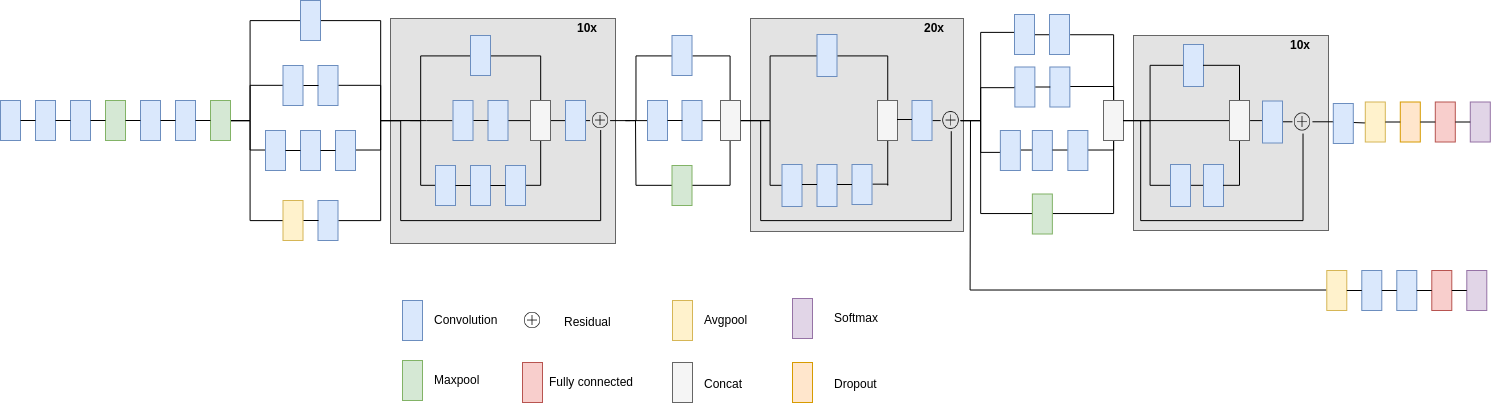
\includegraphics[width=1\textwidth]{methodology/figures/Schematic-diagram-of-InceptionResNetV2.png}
     \caption{The compressed view of the InceptionResNetV2 network inspired by Mahdianpari et al.}
     \label{fig:IRV2}
\end{figure}
\begin{figure}
     \centering
     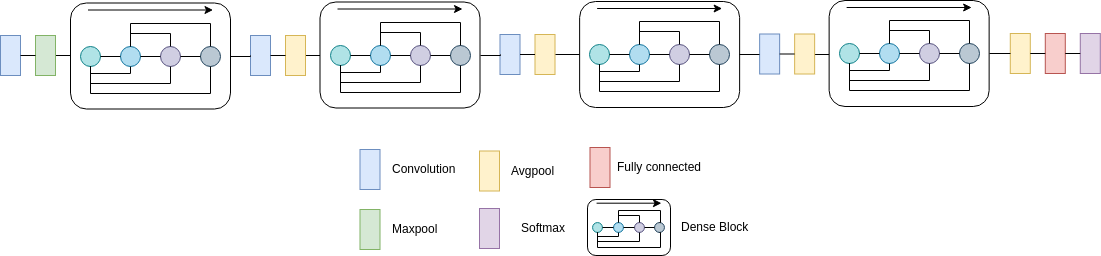
\includegraphics[width=1\textwidth]{methodology/figures/Schematic-diagram-of-DenseNet-model.png}
     \caption{The compressed view of the DenseNet network inspired by Mahdianpari et al.}
     \label{fig:DN}
\end{figure}

Finally, combining the inception and residual modules, we end up with the modules used in InceptionResNetV2. 
Here we combine the strength of both networks. A compressed view of the network is shown in Figure \ref{fig:IRV2} as shown in the article by Mahdianpari et al.~\cite{rs10071119}


\paragraph{DenseNet architecture}
Huang et al. published the DenseNet architecture, as shown in Figure \ref{fig:DN}, with the same goal as InceptionResNet, namely to reduce network size and to get better classification accuracy from a better gradient flow~\cite{Huang_2017}.
In the DenseNet model, all layers are connected in a way to ensure the maximum flow of information between layers. The network achieves this flow by letting each layer convey all its information to all subsequent layers with similar dimensions. This gradient flow gives the network the ability not to store redundant information, and Huang et al. showed significant results for classification with small training datasets where overfitting often would serve a problem.



\subsection{Pooling and Freezing}
The pretrained networks were initially trained for the 1000 classes in the imagenet dataset. Without modifying the network, it would output one of the 1000 classes when confronted with an image. In this thesis, this is not desirable since none of the original classes is usable for medical image classification~\cite{imagenet_cvpr09,imagenet}.
When we introduce our pretrained network, we cut the last two layers from the model and introduce a pooling layer instead.
The two layers cut are the fully connected layer with 1000 nodes, and a softmax layer (The Purple and The Red blocks at the right side of the networks in Figure \ref{fig:IRV2} \& \ref{fig:DN})
As we recall from section \ref{cha:pool}, it is common in the practice of transfer learning to add a pooling followed by a fully connected layer and a softmax layer as a substitute for the original layers removed.  The pooling can either be average or max pooling, and we have the option of using global or local pooling. 

Another prominent way to improve the performance of transfer learning is freezing the layers in the model. When we freeze a layer, we lock the weights of the layer making it not trainable.
The main consequences of freezing layers are related to time and accuracy. 

If we freeze all layers but the last five, the network only has to backpropagate the gradient five steps, reducing the computation time drastically in an extensive network like Densenet. 
By freezing weights, we obviously can not learn anything new with the frozen weights, which means that we can only store new information in the latest unfrozen layers. For similar datasets, this might not be a notable problem, given that they most likely have similar features. When the dataset differs a lot from the transfer learning dataset, we might not reach an optimal solution, given the smaller feature space.





\subsection{Configuring the Optimal Combination for Our Testing}
Based on the article by Huang et al.~\cite{Huang_2017}, we believe that the densenet model would give us the best result. As stated, the densenet model has good gradient flow, and the architecture helps small datasets with overfitting. 
We have also decided to use global average pooling as our pooling layer for both models. We base our decision of the usage of global average pooling on the models used in the Mediaeval workshop by Hicks et al.~\cite{26207} and Borgli et al.~\cite{runeMedico2018} whom both got great results when using global average pooling on medical image data.


\subsection{Summary}
We have, in this section, talked about how we want to use transfer learning to help with the classification. We have looked at the two main advantages with transfer learning, namely the time saved in training and the accuracy gained during evaluation. The advantages coupled with the fact of the widespread use of transfer learning makes it the best option for us, compared to regular classification.
 We then took the results from the SAGA tool made by Borgli et al. and used the most optimal network as our primary network in this thesis. 
In addition to the best network, based on hyperparameter optimisation, we used InceptionResNet as a secondary network for evaluation, reasoning that the use of a generally good network would yield a scenario closer to the real world.
After a brief discussion about the composition of the networks, we concluded with the DenseNet model with global average pooling would yield the best result based on our datasets.





\section{Libraries} 
With the general structure of the algorithms discussed, we will now go more in-depth into the libraries used in the creation of the programs.

In this section, we will discuss the foundation of our code, important external and internal libraries, and the setup and execution of our project.  
We first discuss the programming language in question, give insight into the reasoning behind it. Then we will look into the framework used for machine learning, and in detail how it implemented in our programming language. Lastly, we look into the wrapper we use to get a higher level of abstraction over our code, together with custom functions that are in use by our wrapper. 

\subsection{Python}
When doing machine learning, some of the most popular languages, in no particular order, are Python, Java, R, C++, SQL, and C \cite{kaggle}. Some of these languages, like C and C++, are chosen for their speed, which is often a significant factor in Machine learning. Other languages, like R, is chosen because of its integration into the scientific community long before machine learning became a trend. The last group, consisting of Java and Python has gained popularity because of its already big user base and user-friendliness. Python is also the winner when it comes to machine learning because of, like R, its integration into the scientific community. 
Right now Python is the leading language for machine learning. Driven by this, there is considerable focus into making it faster, to compete with already fast languages, like the C family. 

Python is an interpreted, high-level, general-purpose programming language created in 1991.   It, like many other modern languages, is object-oriented and supports functional programming. 
Mainly because of the excellent support when it comes to machine learning, and the general "easy to use and no compiling" we have chosen python as the base for our code in this thesis. 



\subsection{Tensorflow}
Arguably the biggest reason for the success of machine learning in python lies in Tensorflow~\cite{tensorflow2015-whitepaper}. Tensorflow is a machine learning package released by Google in November 2015 and has since then become the leading framework for machine learning worldwide~\cite{kaggle}.  
Tensorflow is in use by companies like AMD, Twitter, eBay and Snapchat. 


Tensorflow is today a multi-language tool, but it had its origin in python. It is just in later years that other languages have gotten tensorflow support.  
The data flows through a graph network, where the objects in the graph describe the mathematical operations used in the machine learning, and the edges between graphs are the multidimensional arrays storing the weights associated with the operation in question. The name Tensorflow is a combination of the flow we experience during calculation and the tensors between the mathematical operations. 

As stated, Python, and subsequently machine learning in Python, would be much slower than a counterpart in C. Because of this, Tensorflow works as a layer of abstraction to code running in the C language. 
In addition to the layer of abstraction, Tensoflow can do the computation using a graphical processing unit (GPU). Using a GPU for machine learning will often give a considerable speedup to the training, given that the GPU is designed with matrix multiplication in mind. This gives the GPU the option to easily calculate large chunks of the data in a fraction of the time.

Other packages for machine learning like PyTorch~\cite{paszke2017automatic} and Microsofts CNTK~\cite{Seide:2016:CMO:2939672.2945397} would be other options, but as they are not as widespread. Because of the widespread usage, we have chosen to use Tensoflow as our primary machine learning package.



\subsection{Keras}
One of the least attractive things with tensorflow is its unnecessary complexity.  Even though Tensorflow offers more abstraction compared to running the code in pure C, the Tensorflow library can be unnecessarily complex. As a result of this, many external libraries try to simplify many of the complexities that accompany tensorflow. 
Libraries like TFlearn is a modular and transparent deep learning library on top of tensorflow. It gives a higher-level API to Tensoflow to reduce complexity and speed up experiments~\cite{tflearn2016}.
The most successful library for on top of Tensorflow is Keras~\cite{Keras.io}. 
Just as TFlearn, Keras is a high-level package written in python. It is capable of running on top of TensorFlow, CNTK, or PyTorch, which is the tree most popular machine learning libraries at the time of writing.  Keras is made to be user-friendly, modular, easily extensible, and to work with python.

One of the core elements of Keras that makes it a better choice than just running, for instance, Tensorflow, is the concept of a model. A model in Keras is a way to organise the layers of the network in a more organised way, giving a better understanding of how the network is set up, and how each layer type contributes to the graph. 

This thesis relies on Keras as a wrapper for tensorflow. As stated, the use of models and the simplicity of the language makes it an excellent choice of such a large project. Also, Keras has good support for convolutional operations which is the most used methods when managing images. Keras also has the most popular pretrained convolutional neural network models available in its package.





    
\section{Custom Functions for Keras, Tensorflow and Python}
In addition to the standard functions and packages provided by Python, Tensorflow and Keras, we present a list of packages designed during the thesis. A majority of the packages is implementations of leading methods already in place in machine learning, though all methods are redefined to work within the scope of this thesis.
The methods presented have all undergone testing during the thesis, though not every method ended up in the finished product.


\subsection{Channel Wise Fully Connected Layer}
\label{cha:CWDense}
A problem often encountered when working with autoencoders which are not undercomplete is the fact that they learn to represent the data flawlessly~\cite{OvercompleteAE}.
When this problem arises, the network does not learn the fundamental features that define the dataset and instead passes the signal through the network without any consideration of the input data.
This flaw will often defeat the purpose of the algorithm, so data scientists often put in safeguards, like undercompleteness or regulisers, to combat this lack of feature learning. 
This problem extends to other types of generator networks where there are not sufficient compression or regularisation in the layers of the network.
Even though this problem often is solved by compressing the network into a space that can not contain the information correctly, the network does not always learn the features that define the network. 

We propose a custom ``channel-wise fully-connected layer'' in Keras to help with the problem of correctly learning features. This layer is based on the work done by Pathak et al. in their paper on context encoders~\cite{Pathak_2016}.
The channel wise fully connected layer is primarily used in the GAN to transfer information within each feature map, without using convolutions to do it. As we recall, fully connected layers are often not suitable because of the large size of the weight layer associated with it. This layer is essentially a fully connected layer with groups, where the goal is to propagate the information within each feature map.
Given the latent space of $n \times n$ with $m$ feature maps, by not connecting the feature maps together in the fully connected layer we achieve a parameter reduction from $m^2n^4$ to $mn^4$ (ignoring bias terms)~\cite{Pathak_2016}.
With the ``channel-wise fully-connected layer'' the network can learn features from the entirety of the image, and not just local regions as it would with just convolutions. 
Listing \ref{listing:CWDense} shows the source code used for the channel-wise fully-connected layer. The code is presented in the standard way Keras structure its layers. 

%\begin{minipage}{\linewidth}
\begin{listing}
\lstinputlisting[language=python]{methodology/CWDense.py}
\caption{The channel-wise fully-connected layer source code}
\label{listing:CWDense}
\end{listing}
%\end{minipage}

\subsection{Subpixel}
When working with the generative adversarial network, we wanted to achieve more realistic representations at a reasonable image size. 
Making large scale images in generative adversarial networks has been a challenge that has only recently been cracked~\cite{DBLP:journals/corr/DentonCSF15}~\cite{DBLP:journals/corr/abs-1809-11096}.
As an early measure to fix this problem, we experimented with the use of a Sub-pixel layer as presented by Shi et al.~\cite{DBLP:journals/corr/ShiCHTABRW16} to give a more realistic output compared to just a standard conv-tanh layer.

During this thesis, we have done multiple tests with this layer. In the datasets used for evaluation, we did not end up using any Subpixel layers.

\begin{figure}[b]
\centering
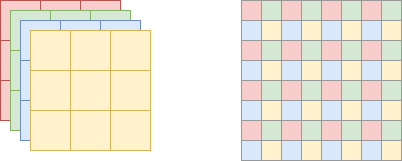
\includegraphics[scale=0.8]{methodology/figures/SubPixel.png}
\caption{How the layers in the sub pixel layer is stacked. Recreated from the SubPixel paper by Shi et al.~\cite{DBLP:journals/corr/ShiCHTABRW16}}
\label{fig:SubPixel}
\end{figure}


\subsection{Masklaod and Setload}
The default way of loading data into Keras is with the usage of the default generators provided by their library. The Keras.ImageDataGenerator() does an adequate job when loading images, though it had some shortcomings.
Maskload and Setload are custom loaders we made for this thesis to get a more simple way of loading, augmenting, and storing images.

Maskloader has the primary job of adding and removing masks from images. In addition to masking, it can flip and mirror the images. Maskloader can mask text in images, though at a timeframe not feasible for this thesis at a time up to two seconds per image. 

Setload is a library for loading a large number of images for training. In addition to loading images, we designed Setload to remove black borders from images if necessary. 
We use morphological opening\footnote{Morphological opening is the dilation of the erosion of an image } to remove any nonblack pixels in the edges of the image that original from text added post-capture, which gives ut a clean cut as close to the ´´true'' image as possible. The Setload function defaults to normalise the images around zero. This normalisation is to stabilise both the GAN and AE.


\subsection{Self Attention}
\label{cha:attention}
There are features in the images that are more important than others. One of the things we often want to preserve when we recreate images are hard edges. To get a semantically meaningful image,  we often want to differentiate between background and the mucous. 
To see if the network can learn the features needed we are introducing the Self Attention layer to help with this. We base the self-attention on the work done by Zhang et al.~\cite{DBLP:journals/corr/selfattention}.

Self attention for the purpose of this thesis is a tool that the GAN can use to better focus on certain parts of the image. 
In our testing, self attention was used with a residual connection to prevent the layer from destabilising the model. We do not use self attention in the final datasets used for evaluation.

%\begin{minipage}{\linewidth}
%\begin{listing}
%\lstinputlisting[language=python]{methodology/SelfAttention.py}
%\caption{The self attention layer source code}
%\label{listing:Attention}
%\end{listing}
%\end{minipage}

\begin{figure}
\centering
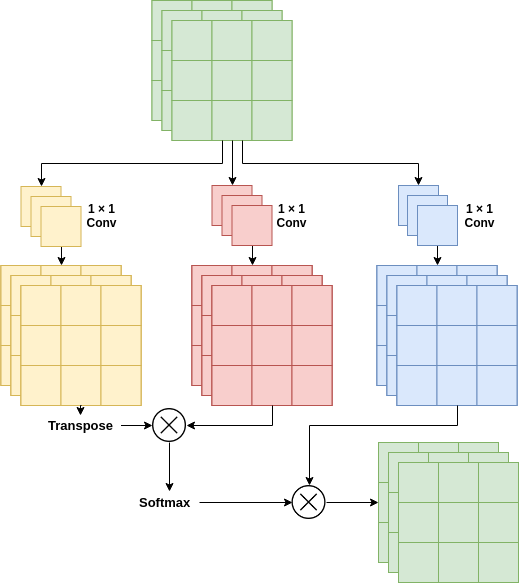
\includegraphics[scale=0.4]{methodology/figures/attention.png}
\caption{How the layers in the Self-Attention layer is stacked. Recreated from the Self-Attention paper by Zhang et al.~\cite{DBLP:journals/corr/selfattention}}
\label{fig:Attention}
\end{figure}



\subsection{Masked loss}
A problem encountered for both the autoencoder and the GAN is what happens when the non-inpainted area gets too close to correct ground truth. 
As most of the image remains unchanged between the input-output space, the loss for most of the image approaches 0 while the inpainted area stays at a high loss value for most of the training. 
As we recall from section \ref{cha:convNet}, we store our data as float32, and as the loss gets smaller and smaller, the squaring of the float32 gives at some point a number so small that the loss flips to a large integer and subsequently ruins the run\footnote{This flipping is at this time our best theory concerning the sudden spike in the loss as it gets closer and closer to zero.}. 

To improve the stability of the training, we have modified the loss to only apply to the areas we inpaint, leaving the rest of the image without a gradient to improve itself. Listing \ref{listing:maskedMSE} shows the source code for the masked MSE. 
For each point in the MSE we apply a binary mask. If the binary mask is zero, we do not consider that space during backpropagation.


The masked loss showed a considerable increase in stability during training, but in the finished product, we only used it for the autoencoder when we struggled with stability problems.

\begin{minipage}{\linewidth}
\begin{listing}
\lstinputlisting[language=python]{methodology/maskedMSE.py}
\caption{The self attention layer source code}
\label{listing:maskedMSE}
\end{listing}
\end{minipage}





\section{Stabilising the GAN}
Before we ended up with the model we used in the thesis we ran multiple experiments to make the generative adversarial network stable for training.  In contrast to the autoencoder, the GAN does not use the ground truth as a reference point. Where the autoencoder always has a gradient based on the input data, the generator in the GAN gets its learning gradient from another network.

This lack of a ground truth gives the GAN many pitfalls that cause the training process to crash \footnote{Crashing is not the right word to use, but the result is the same: The learning process stops.}.


\paragraph{Normalise the inputs}
One of the first measures we did to prevent training collapse was to normalise the inputs. Instead of using images in the range 0 to 255 in pixel values we switched the values to  -1 to 1. 
Later, when the images were generated, we switched out the standard sigmoid output layer with a tanh output layer. As we wanted the output to be between -1 and 1, this was necessary, as the sigmoid only outputs between 0 and 1.

\paragraph{Using Gaussian noise}
When generating noise for the generator model, we only sample from a Gaussian distribution and not a uniform distribution. We base the reasoning on previous work in the generative modelling field of research.

\paragraph{Permanent Dropout}
A measure we took to improve stability were to use permanent dropout~\cite{DBLP:journals/corr/IsolaZZE16}. We used the same amount of dropout both during training and testing.
The usage of dropout, in general, was a quintessential part of stable GANs, but in the end, we did not end up with permanent dropout in the finished model.


\paragraph{Normalising the batches}
One of the most significant challenges we encountered when training the adversarial network was the use of correct normalisation. 
The practice of individually training the discriminator with real and fake samples gave higher stability overall compared to a mix during training. 
The use of instance normalisation gave a better result compared to using batch normalisation. We believe this is contributed to the fact that the discriminator learned that the average pixel value was lower for the whole batch since the area inpainted had 0 as the pixel value.
The final model ended up not using batch or instance-normalisation except for in the discriminator. 



\paragraph{Avoiding sparse and vanishing gradients}
Most of the well-known networks use the ReLu\cite{Nair/2010/RLU/3104322.3104425} activation function \cite{DBLP:journals/corr/SimonyanZ14a} \cite{DBLP:journals/corr/SzegedyIV16} 
\cite{DBLP:journals/corr/HeZRS15}.
We saw the best result when we used non-sparse gradients during training. 
Instead of using ReLu we used the slightly modified LeakyReLu \cite{Maas2013RectifierNI}.

In addition to trying to remove sparse gradients, we also wanted to address the problem with vanishing gradients during training. Given that we have fully saturated pixels (with the value of 1) and we have fully darkened pixels (with the value of -1) we, at the end of the experimentation phase, ended up removing the tanh layer. 
The removal of the tanh layer meant that the pixel values could be arbitrary on both positive and negative value, so we had to clip the value not to get an error at test time. 



\paragraph{Avoiding residual and inception layers}
When training the GAN, experiments show that the usage of both residual \cite{Rumelhart:1986:LIR:104279.104293} and inception \cite{DBLP:journals/corr/SzegedyLJSRAEVR14} models do not contribute to a good result when training the GAN.

We recall that residual modules primary strength is that they always send the image/signal throughout the network in addition to the standard layers, making the gradient flow better at the start of the network. 
This modification to the original image might seem reasonable when it comes to inpainting, but in reality, this does not work.  Given an image where we want to change only the inpainted area, the image is about 80\% unchanged. The network could focus on just filling in the inpainted area in theory, but in practice, the network tries to change the rest of the image in addition to the square. This incorrect inpainting gives us a generator that changes too much of the image and a discriminator that does not learn any essential features since the input and output are relatively similar from the start.

Inception modules primary strength is the fact that the gradient can flow throughout the path most suited to the problem at hand.
We tested some training runs with inception modules, but the result was not impactful enough to continue to use this architecture.

From multiple training runs, it seems like just a straight forward encoder-decoder network for the generator yielded the best result while the best result for the decoder was to use convolutions with a stride to downsample the signal.



\FloatBarrier
\section{Code Description}
We have, at this point, gone through the objective of our thesis, and shown how we want our result to be generated and evaluated in practice. 
We will now go more in-depth into the two networks used for generating the new datasets and go in-depth into the model we use for classification.


\subsection{Autoencoder}
The autoencoder we used to generate the datasets used in this thesis bears a resemblance to the standard autoencoder proposed in chapter \ref{cha:Explaining_autoencoders}. Here we use a standard encoder decoder network.

\paragraph{Loss, Optimiser}
To get the autoencoder to give the best result, we have chosen to use the mean square error loss as in equation~\ref{eq:MSE_form} and the Adam~\cite{adam} optimiser.
The mean square error was a logical choice since we already have the ground truth and we only want to recreate the inpainted area based on what used to be there before the masking.
The Adam optimiser was chosen by the widespread usage in machine learning, coupled with the fact that it works well with sparse gradients.

\paragraph{Encoder}
The input to the autoencoder were the masked images at $256 \times 256$ px to compress the information in the encoder we solely used convolutions with a stride of 2. An alternative to using stride for the downsampling would be to use pooling, as described in section \ref{cha:pool}. Both concolution with stride and pooling gives adequate results, though we chose to use convolutions.



\paragraph{Decoder}
Between the encoder and decoder we added a 25\% dropout layer. This layer is the only reguliser in the network, though since the job was to inpaint and not recreate, the autoencoder needed information about a rather large area of the image, and hence had little possibility to overfit.

Upsampling could either be achieved with upconvolution or with upsampling.
Using upconvolution gives the network more variables (as the filters use weights, and upsampling does not), and hence would require more training. 
In this thesis, we achieved the most significant results by using upsampling compared to upconvolution, though we can not rule out that upsampling would be better with more complex images, or at larger image sizes.

\vspace{5px}

To describe the model we will look at the example where we try to inpaint the green square in the image, and nothing else.
To train the autoencoder for inpainting, we divide the dataset in two, first images with the green square and images without the green square. We discard the images with the green square since they are not viable for training.  The resulting dataset will only contain images without green sources. 
\begin{figure*}[]
\centering
\begin{subfigure}[b]{0.45\textwidth}
    \centering
    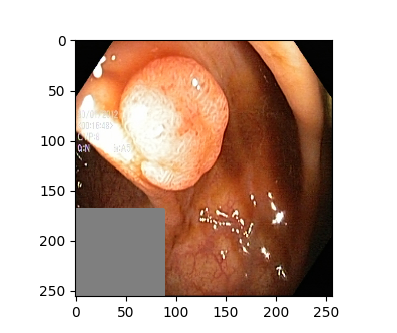
\includegraphics[width=\textwidth]{methodology/figures/masked_img.png}
    \caption{Image the autoencoder receives as an input }    
    \label{fig:AErec}
\end{subfigure}
\hfill
\begin{subfigure}[b]{0.49\textwidth}  
    \centering 
    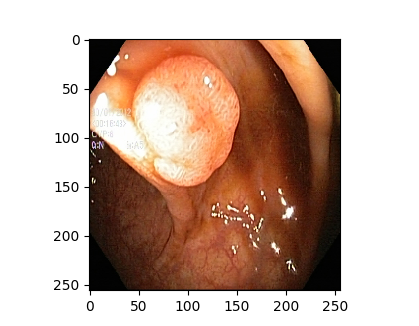
\includegraphics[width=\textwidth]{methodology/figures/whole_img.png}
    \caption[Hate to be this guy]%
    {{\small The missing part the autoencoder tries to replicate}}    
    \label{fig:AErep}
\end{subfigure}
\caption{A standard image taken in by the autoencoder} 
\label{fig:AEmasks}
\end{figure*}

The next step before training is to cut the images according to the mask provided. Figure \ref{fig:AErec} shows what the finished masking looks like, and \ref{fig:AErep} shows what we want to achieve after training.

We feed \ref{fig:AErep} into the autoencoder consisting of the convolutional layers described earlier with primarily leakyReLu layers within the model and a tanh layer at the end.



\subsection{Generative adversarial network}
The GAN used the same generator discriminator elements as the Goodfellow GAN; however, the most significant difference is the fact that our model does not generate the image from Gaussian noise.
Instead of the standard Gaussian noise as input to the generator, the inpainted image is taken as input. 

\paragraph{Discriminator}
The discriminator, as we can recall, had the job of determining if an image is real or fake. As with the decoder in the autoencoder, we can use both pooling and convulsions as downsampling. Here, as in the autoencoder we solely used convulsions with stride as to downsample, with intermittent normalisation. The Normalisation layers helped with the stability issues that we face when training GANs. In the end, we flatten and connect the network to a fully connected node to determine true or false.

\paragraph{Generator}
The generator in the GAN used both up and downsampling with the fully connected dense layer in the middle, as described in section \ref{cha:CWDense}.  
During the five repetitions of downsampling, we added LeakyReLu and batch normalisation and, as before, used convulsions with a stride to compress the network.
Upsampling consisted of upsampling in the same way as in the autoencoder, followed by convolutions, LeakyReLu and a dropout rate of 40\%. 



\subsection{Transfer learning classifier}
We have in section \ref{cha:classifier} gone in-depth into the two desired networks used in this thesis.  Our main objective when making a classifier is to make a system that is robust, reliable and has the option to be modular. 
We built the classifier to gather the same information as shown in Figure \ref{fig:KTLmodel}, meaning we first specify the desired network (VGG~\cite{simonyan2014very}, DenseNet~\cite{DBLP:journals/corr/HuangLW16a}, or Mobilenet~\cite{DBLP:journals/corr/HowardZCKWWAA17}), then we specify the optimiser (NAdam, Adam, RMSprop or SGD).
After the network and optimiser are chosen, the network takes information about the dataset related parameters; batch size, K-folds, Patience, and epochs.

when all variables are determined, the networks train for the desired amount of time for each of the datasets provided.

\begin{table}[h]
\begin{center}
\small
\begin{tabular}{llllll}
\toprule
\multicolumn{1}{c}
{Model}             & Size   & Top-1 Accuracy & Top-5 Acc & Parameters  & Depth \\
\midrule
Xception          & 88 MB  & 0.790          & 0.945          & 22,910,480  & 126   \\
VGG16             & 528 MB & 0.713          & 0.901          & 138,357,544 & 23    \\
VGG19             & 549 MB & 0.713          & 0.900          & 143,667,240 & 26    \\
ResNet50          & 98 MB  & 0.749          & 0.921          & 25,636,712  & -     \\
ResNet101         & 171 MB & 0.764          & 0.928          & 44,707,176  & -     \\
ResNet152         & 232 MB & 0.766          & 0.931          & 60,419,944  & -     \\
ResNet50V2        & 98 MB  & 0.760          & 0.930          & 25,613,800  & -     \\
ResNet101V2       & 171 MB & 0.772          & 0.938          & 44,675,560  & -     \\
ResNet152V2       & 232 MB & 0.780          & 0.942          & 60,380,648  & -     \\
ResNeXt50         & 96 MB  & 0.777          & 0.938          & 25,097,128  & -     \\
ResNeXt101        & 170 MB & 0.787          & 0.943          & 44,315,560  & -     \\
InceptionV3       & 92 MB  & 0.779          & 0.937          & 23,851,784  & 159   \\
InceptionResNetV2 & 215 MB & 0.803          & 0.953          & 55,873,736  & 572   \\
MobileNet         & 16 MB  & 0.704          & 0.895          & 4,253,864   & 88    \\
MobileNetV2       & 14 MB  & 0.713          & 0.901          & 3,538,984   & 88    \\
DenseNet121       & 33 MB  & 0.750          & 0.923          & 8,062,504   & 121   \\
DenseNet169       & 57 MB  & 0.762          & 0.932          & 14,307,880  & 169   \\
DenseNet201       & 80 MB  & 0.773          & 0.936          & 20,242,984  & 201   \\
NASNetMobile      & 23 MB  & 0.744          & 0.919          & 5,326,716   & -     \\
NASNetLarge       & 343 MB & 0.825          & 0.960          & 88,949,818  & -        \\   
\bottomrule
\end{tabular}
\end{center}
\caption{Models provided by Keras}
\label{tab:Kaeras_app}
\end{table}

Table \ref{tab:Kaeras_app} shows the pretrained networks available to load in the Keras framework. 
When training we did some extra steps at the end, namely added global average pooling and a fully connected layer with the desired number of outputs (usually eight classes, and eight outputs)


\section{Summary}
In this chapter we have, in more detail, looked at the process and purpose of inpainting and classifying.
We started with the discussion regarding where to inpaint, and the problem statements we wanted to test for each of the inpaintings. 
We made a decision regarding if inpainting of the test set were feasible, and decided the two types of generative modelling algorithms we use in this thesis. 
We looked at the need for a classification model to discern the results of our inpainting and decided to use transfer learning to represent a real-world scenario better.
We looked into the two transfer learning models we use in this thesis, namely Densenet121 and InceptionResNetV2, and gave a brief overview of their similarities and differences.

After a more conceptual view, we talked more about how we would achieve the experiments in practice.  Here we talked about why we chose python, tensorflow and keras, followed by custom functions needed for our machine learning algorithms. 
We ended the chapter with the description of the three models in practice.

 
